\section{Indaband}
A música, enquanto atividade e produto, permite o estabelecimento de laços sociais
entre musicistas e ouvintes.

A atividade musical permite que um conjunto de musicistas interaja e
comunique-se, facilitada quando os membros compartilham de uma mesma bagagem
cultural. Além disso, permite que a audiência estabeleça um vínculo com
o músico executor ou o conjunto de musicistas \cite{cook2021music}.

Por sua vez, a música enquanto produto permite o estabelecimento de laços sociais
entre os ouvintes, seja em uma sala de concerto no século XIX, em uma sala de estar
com um rádio ou um gramofone no século XX, ou em uma apresentação ao vivo na
plataforma Twitch no século XXI.

Durante a pandemia de COVID-19, estudantes de música precisaram adaptar seus
hábitos de prática musical para aulas remotas e práticas individuais. A prática
coletiva foi fortemente afetada, uma vez que as aulas e os ensaios presenciais
foram suspensos em uma série de instituições de ensino, dado o risco de
contaminação e a necessidade de distanciamento social \cite{nusseck2021musical}.

A prática remota síncrona, hoje, enfrenta uma série de desafios técnicos. A
latência entre os praticantes é o principal problema. O limiar da percepção
auditiva para atrasos é de cerca de 20 milissegundos, enquanto que sistemas VoIP
com latência de 150 milissegundos e \textit{jitter} de 30 milissegundos são
considerados de boa qualidade. A codificação associada à compressão do sinal e a
largura de banda também influenciam no atraso. Enquanto a latência em uma
comunicação instantânea não for inferior ao limiar da percepção, essa forma de
prática musical não será viável.

A principal alternativa é a prática musical colaborativa assíncrona. Nesse
cenário, cada praticante grava sua faixa de forma individual enquanto ouve as
demais faixas gravadas. Aplicações como \textit{BandLab}, \textit{Ableton Live}
e \textit{Soundtrap by Spotify} funcionam sob essa abordagem.

Uma segunda característica da prática musical coletiva, seja no contexto
presencial ou remoto, é a necessidade de encontrar outros interessados com
gostos musicais similares, instrumentos que se complementem, etc. Uma pessoa que
deseja tocar um estilo musical específico, incomum na região em que vive,
sofreria dessa dificuldade. Um meio de resolver esse problema é recorrer à
comunidades virtuais ou redes sociais. Ao encontrar outros interessados, caso a
distância impeça a prática presencial, a atividade pode ser realizada a partir
da prática musical colaborativa assíncrona. Plataformas como \textit{Cifra Club}
e \textit{Ultimate Guitar} permitem que usuários contribuam com tablaturas de
músicas e comentários, formando uma comunidade virtual.


Tanto a prática musical colaborativa assíncrona quanto a formação de comunidades
virtuais de música são problemas os quais o mercado oferece poucas soluções
integradas. Estações de trabalho de áudio digital (DAWs, do inglês
\textit{Digital Audio Workstations}) mais tradicionais, como \textit{Pro Tools},
\textit{Logic Pro} e \textit{Ableton Live} são desprovidos de funcionalidades de
interação social. \textit{Cifra Club} e \textit{Ultimate Guitar} não permitem a
gravação colaborativa de forma assíncrona. \textit{Soundtrap by Spotify} e
\textit{BandLab} permitem a edição colaborativa em tempo real, porém apenas o
último contém funcionalidades de interação e integração social entre usuários. A
aplicação \textit{Collab}, da Meta, preenchia parcialmente esses critérios antes
de ser descontinuada. O aplicativo móvel Indaband foi criado para ocupar esse
espaço pouco preenchido no mercado.

\begin{figure}[h]
    \centering
    \subfigure[]{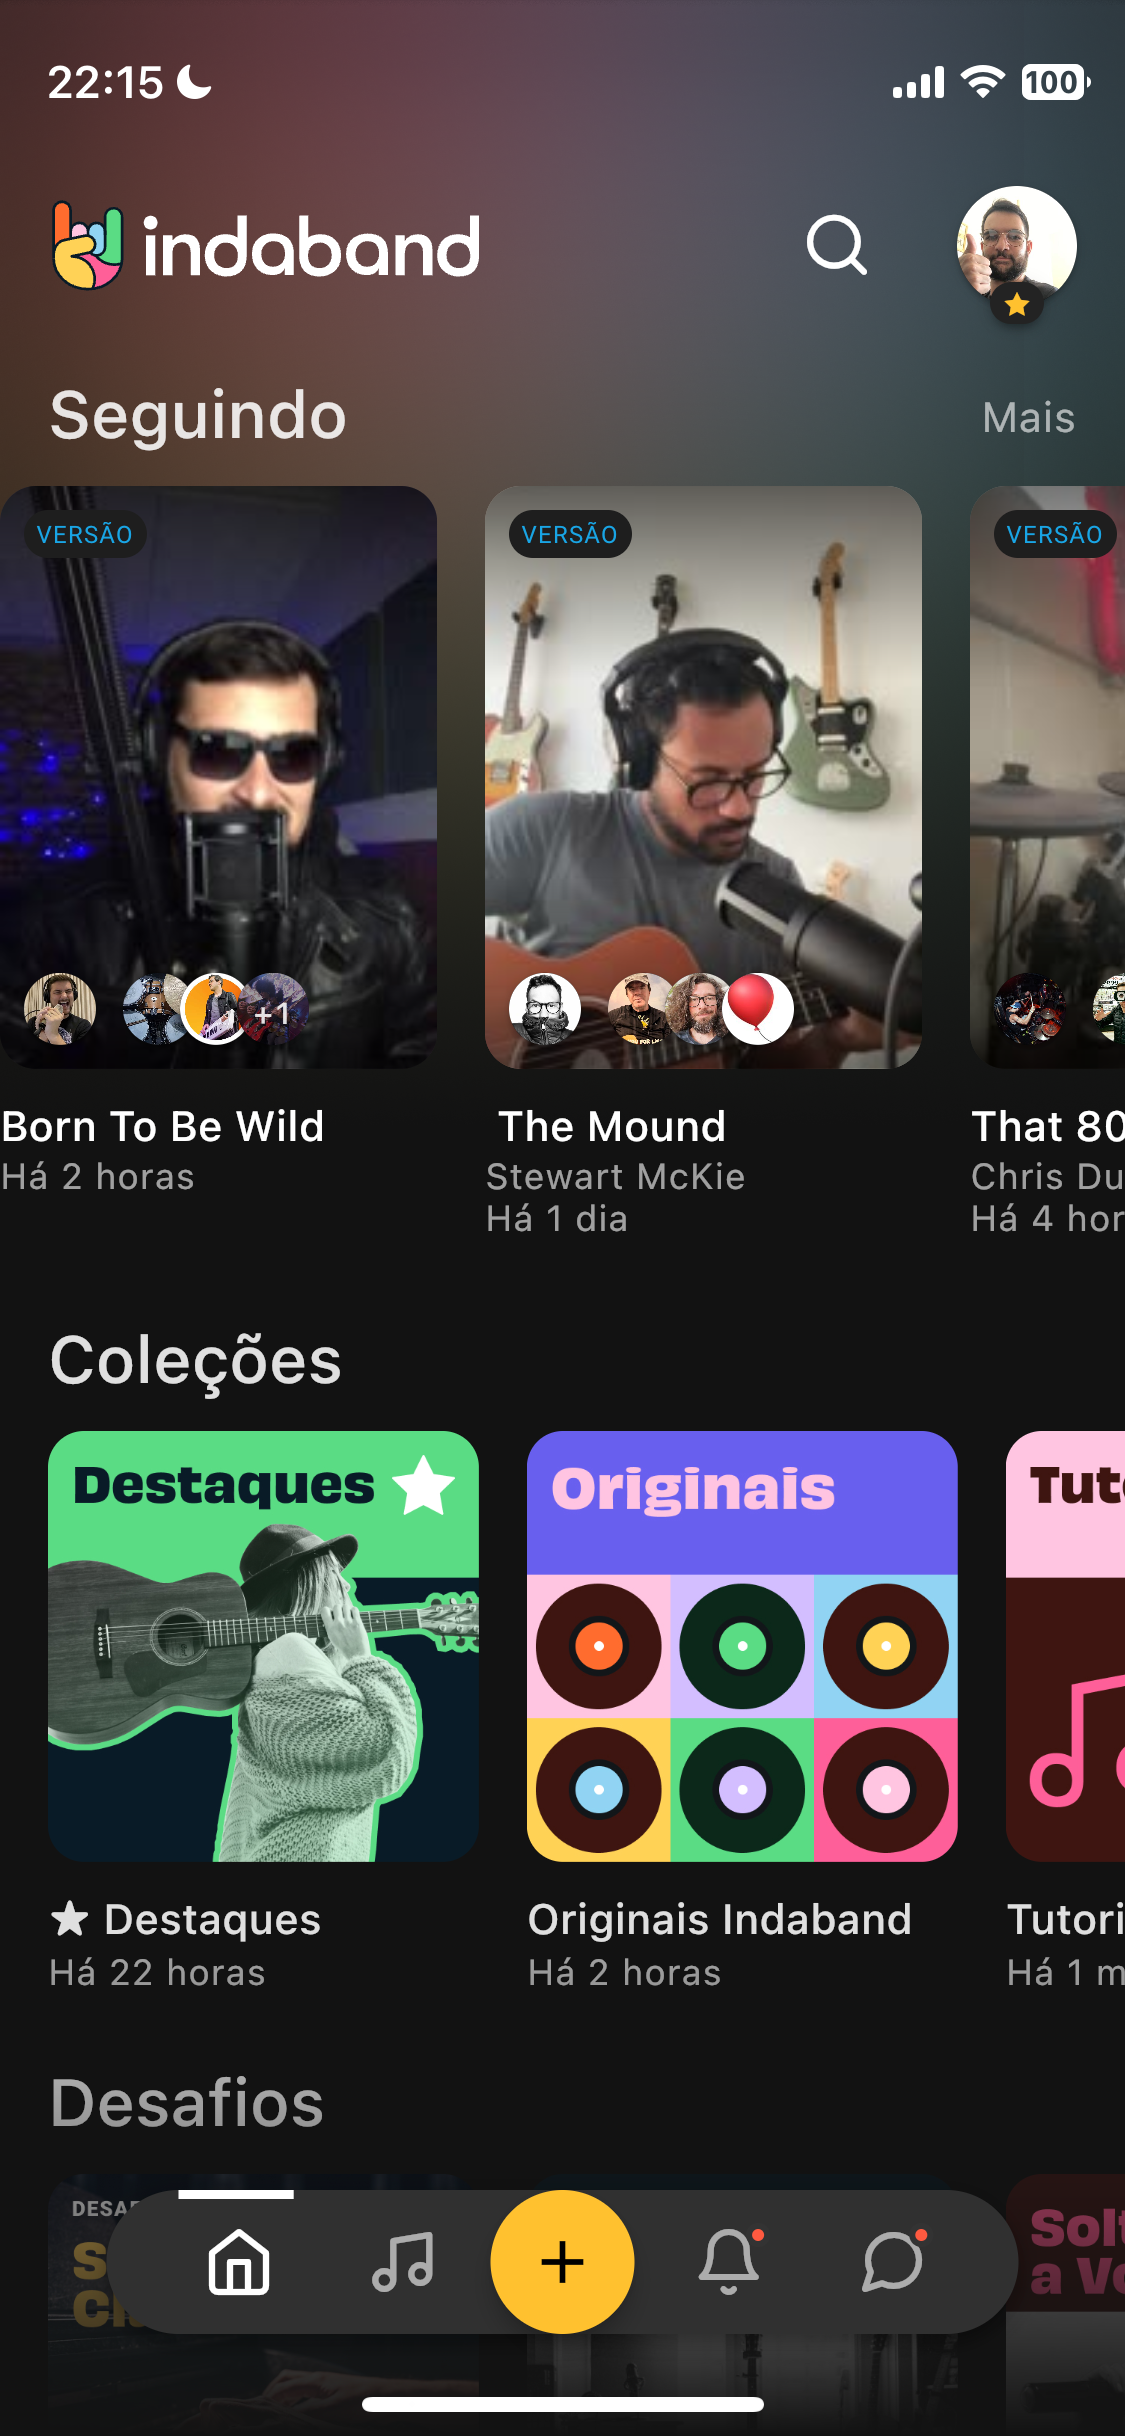
\includegraphics[width=0.24\textwidth]{chapters/chap01/images/inda/inda3.PNG}}
    \subfigure[]{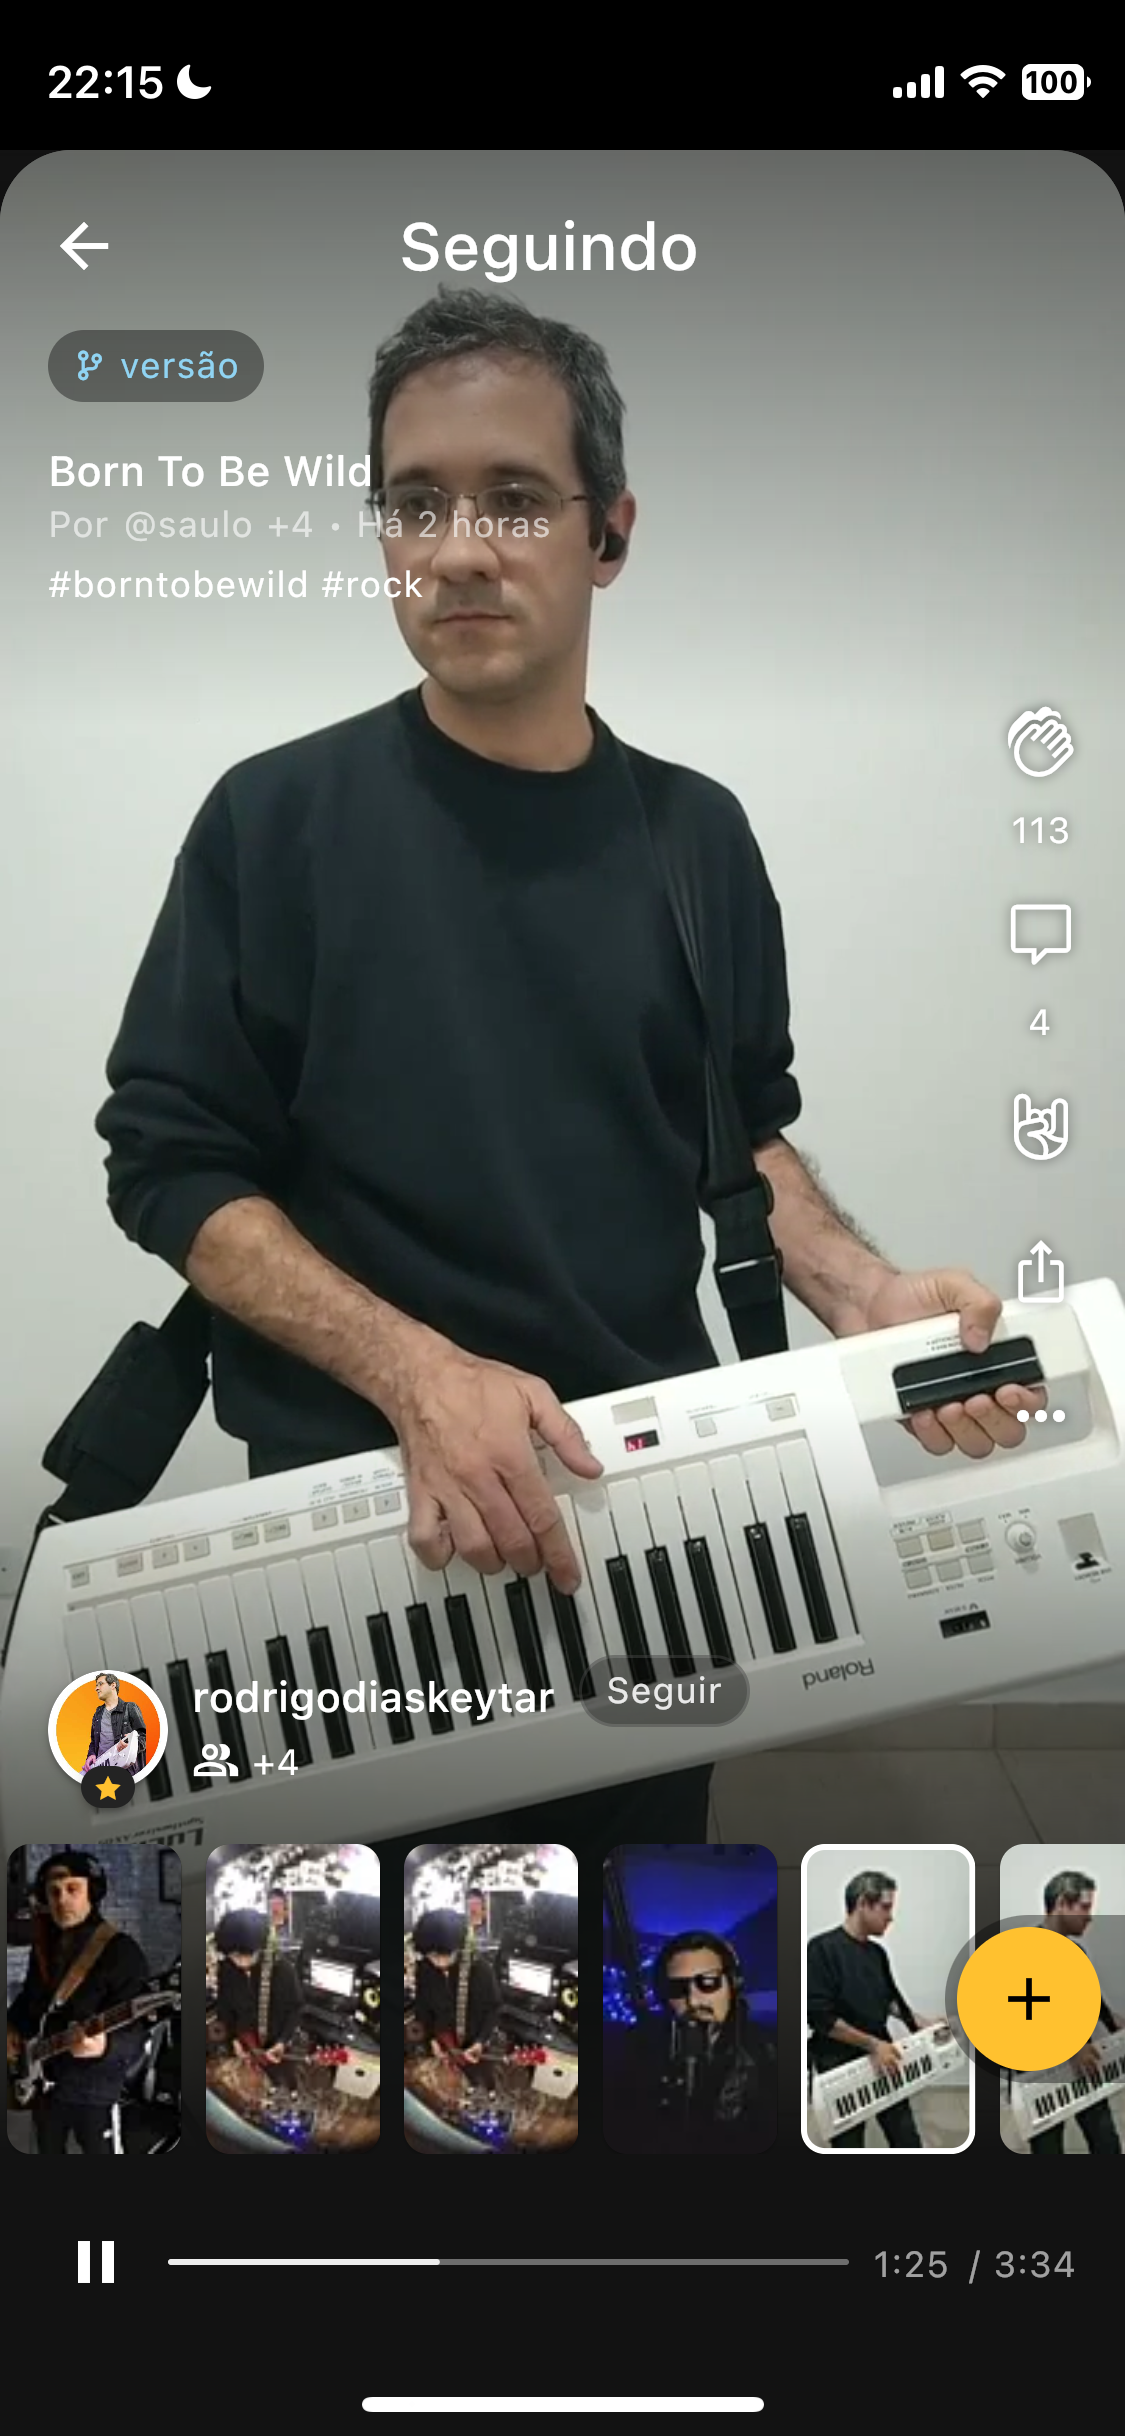
\includegraphics[width=0.24\textwidth]{chapters/chap01/images/inda/inda.PNG}}
    \subfigure[]{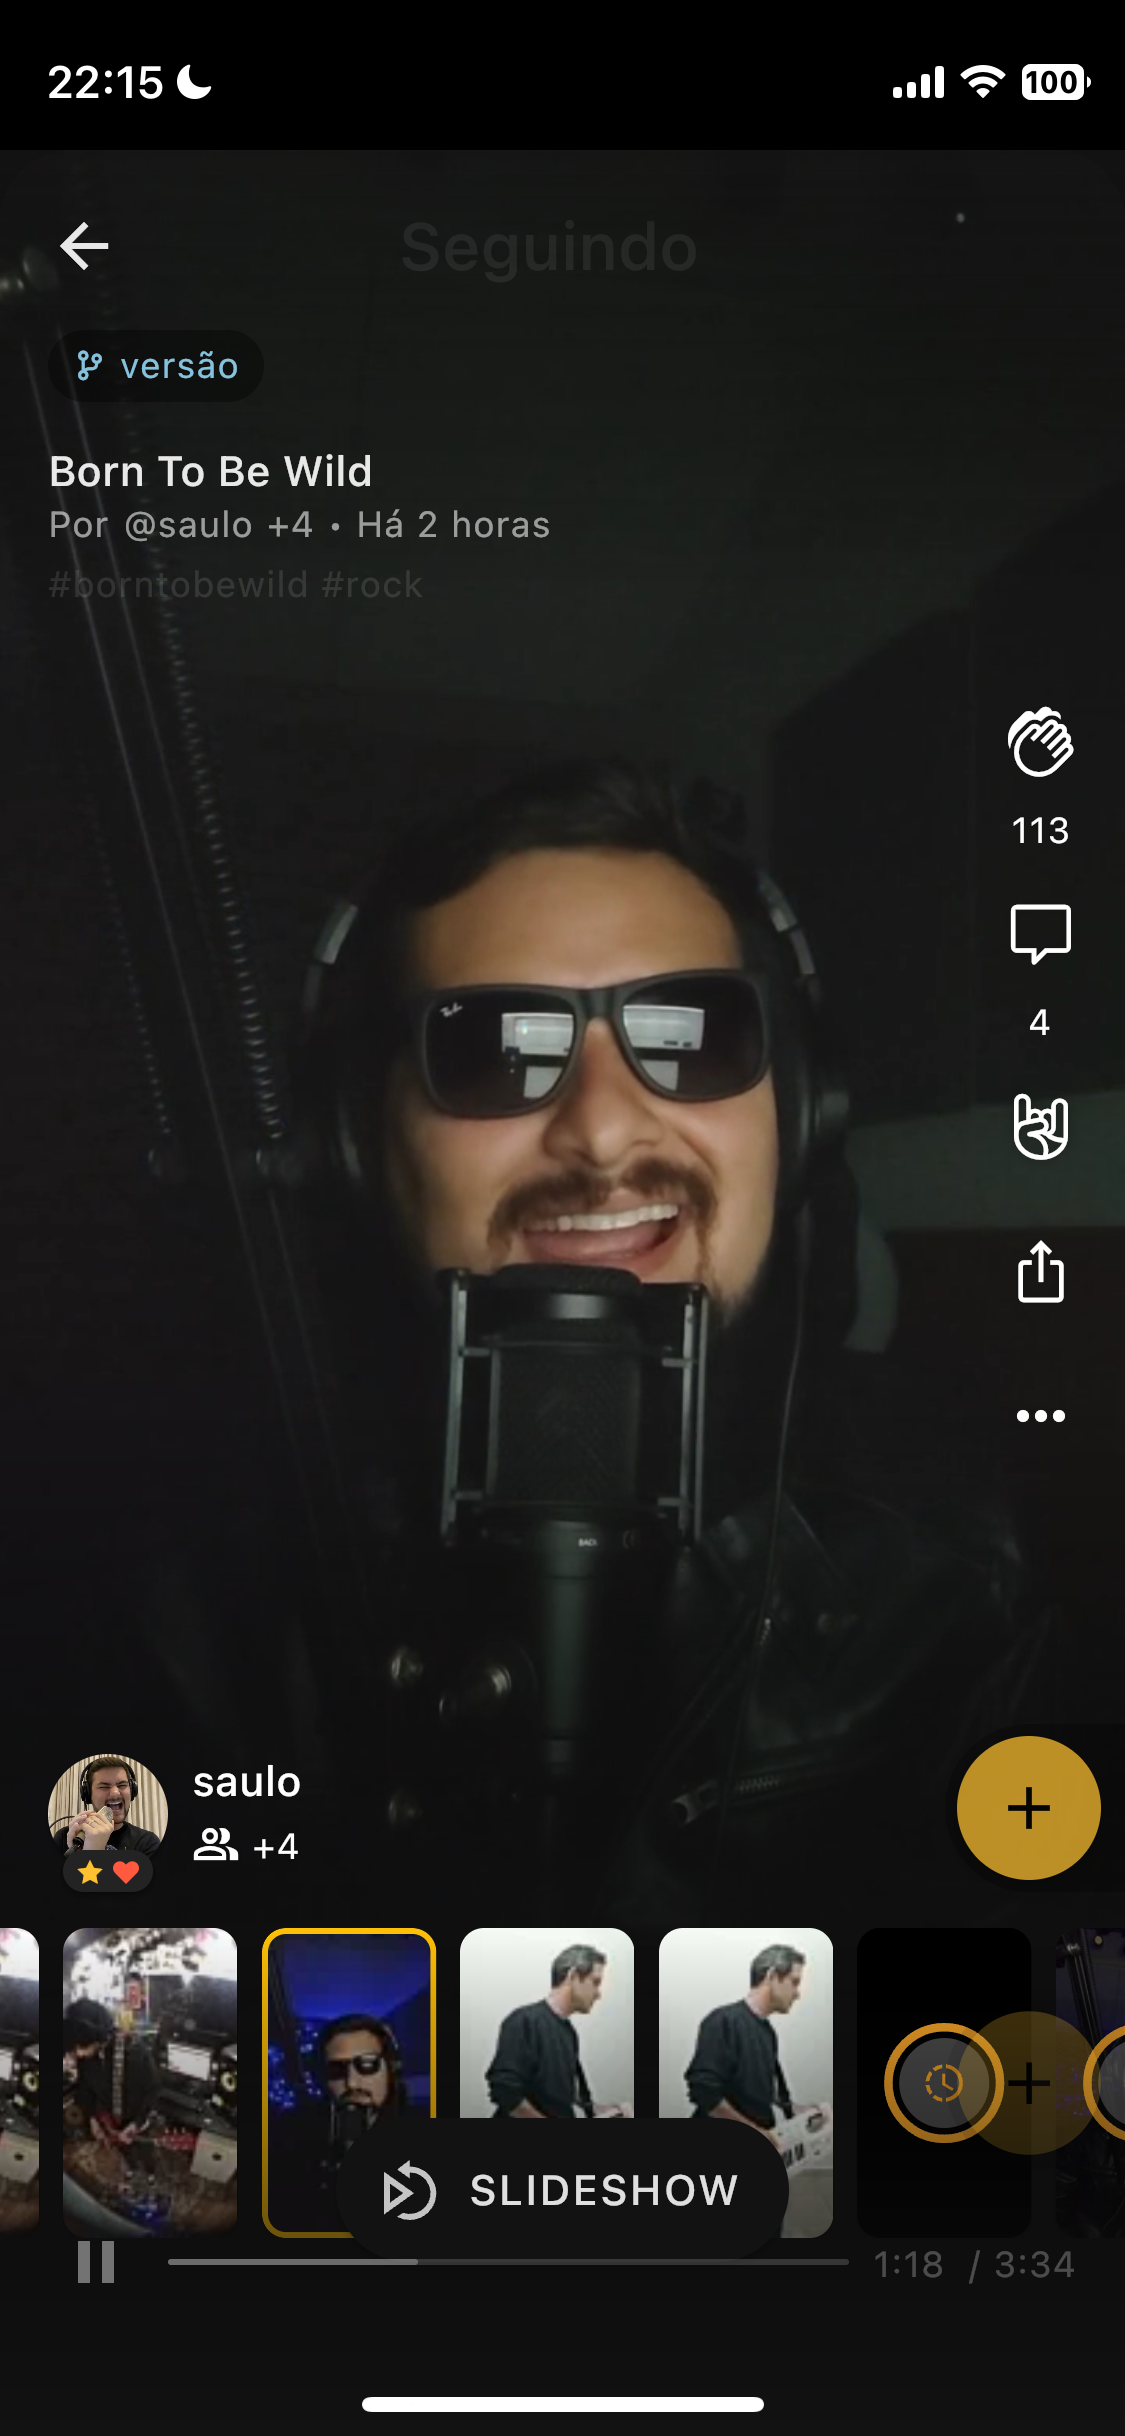
\includegraphics[width=0.24\textwidth]{chapters/chap01/images/inda/inda2.PNG}}
    \subfigure[]{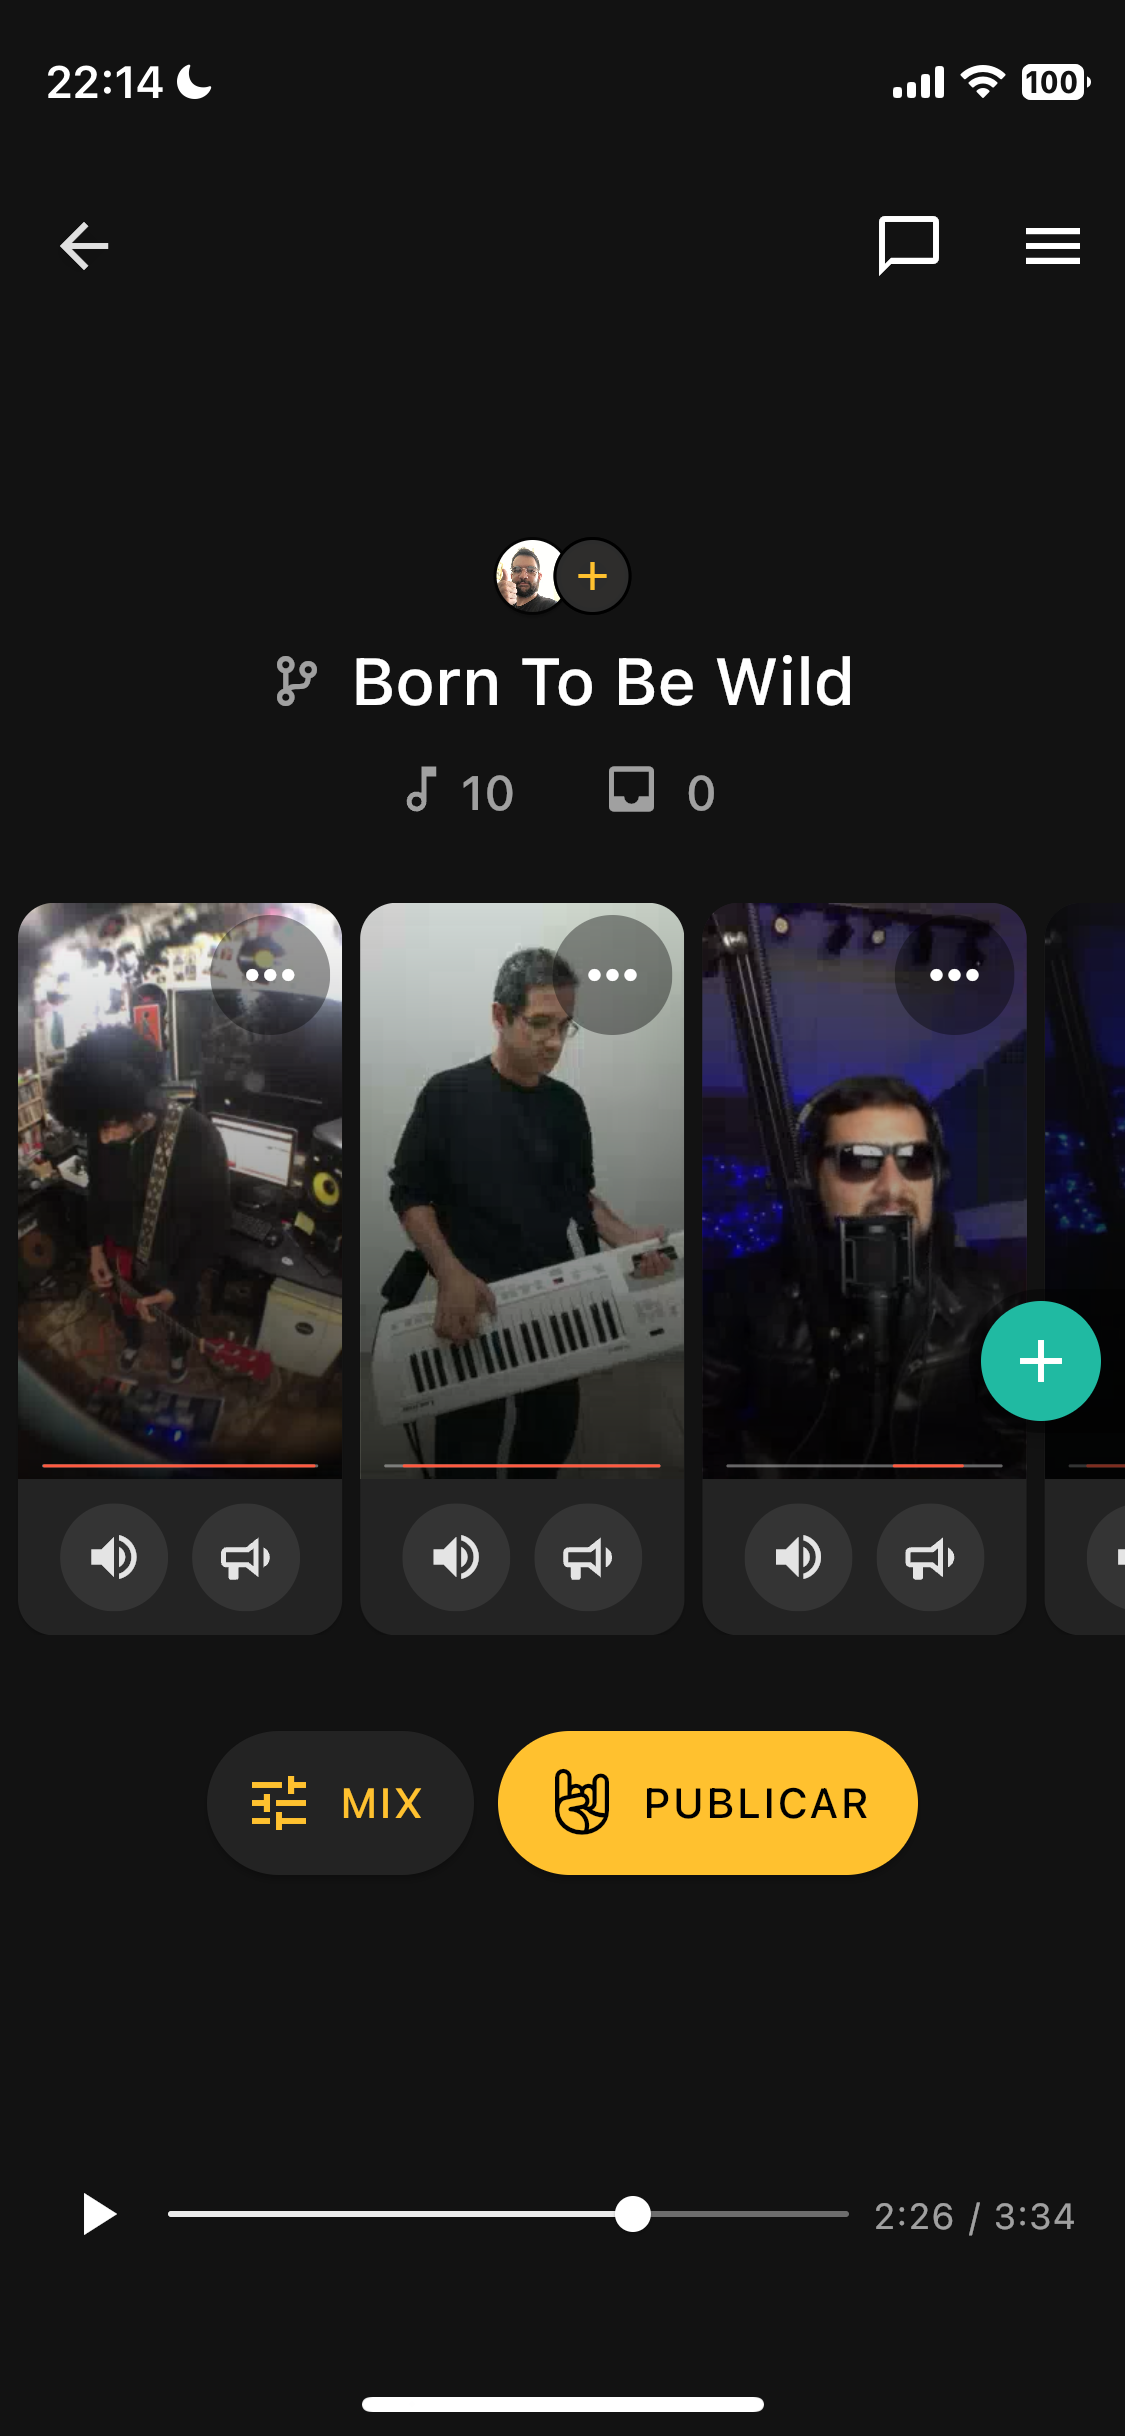
\includegraphics[width=0.24\textwidth]{chapters/chap01/images/inda/inda4.PNG}}
    \caption{Recursos do \textit{app Indaband}: (a) \textit{Home} (b) \textit{Feed} (c)
    \textit{Feed} (d) \textit{Studio}.}
    \label{fig:cap_tela}
\end{figure}

Indaband é uma aplicação móvel para distribuição e gravação de música
colaborativa e remota \cite{indaband}. A versão inicial foi disponibilizada
publicamente em Agosto de 2022. O quadro de funcionários é majoritariamente
brasileiro, enquanto que o produto possui distribuição global. A FIGURA
\ref{fig:cap_tela} exibe capturas de tela da interface visual.

Na aplicação, usuários podem criar sessões, que são ambientes colaborativos de
gravação entre os participantes. As sessões contam com ferramentas para gravação
e mixagem. O ambiente de pré-visualização, edição e produção da sessão chama-se
\textit{Studio}.

Uma vez que o usuário conclua as etapas de produção da sessão no \textit{Studio}
e esteja satisfeito com o resultado final, ele tem a opção de publicar a sessão
no \textit{Feed} público da aplicação. No \textit{Feed}, todos os usuários da
plataforma podem visualizar e interagir com a sessão publicada adicionando
comentários, aplausos e compartilhando com outros usuários dentro e fora da
aplicação.

Após três anos de desenvolvimento, a aplicação conta com dezenas de milhares de
usuários cadastrados, os quais centenas gravam mensalmente. Dado o grande
catálogo de usuários, o processo de encontrar pessoas com interesses musicais
similares demanda tempo e esforço. O mesmo ocorre ao procurar uma sessão que
seja de interesse em meio ao grande volume de conteúdo publicado. Essa
dificuldade percebida pelo usuário é conhecida na literatura de sistemas de
recomendação como sobrecarga de informação \cite{roetzel2019information}.

\section{Sobrecarga de informação}

A sobrecarga de informação, segundo \citet{roetzel2019information}, é um estado em que um tomador de decisões observa um
conjunto ou uma carga de informações de complexidades distintas, a qual inibe a
capacidade do tomador de decisões de determinar de forma ótima a melhor decisão
possível.

\vspace{0.2cm}
\begin{figure}[h]
    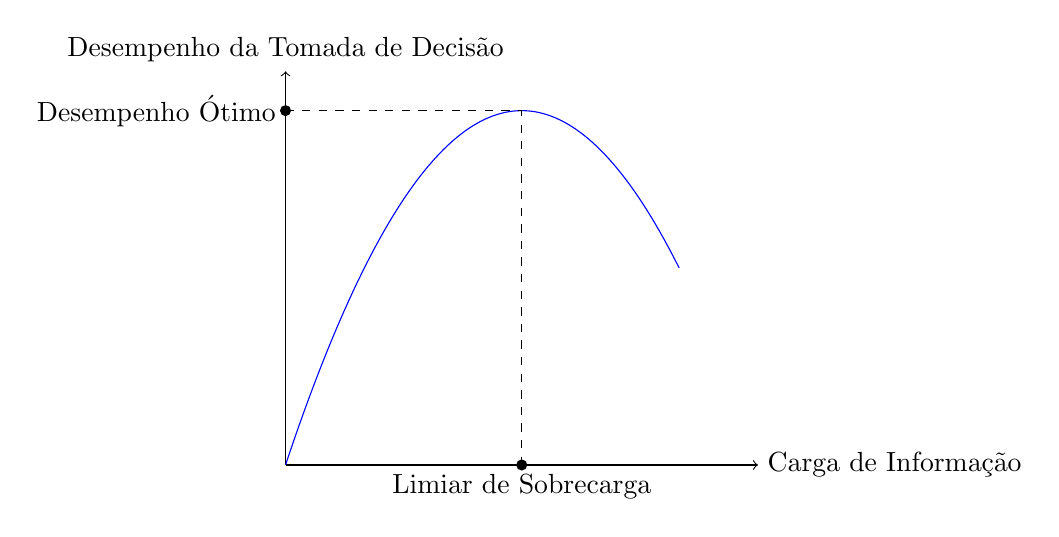
\begin{tikzpicture}
    % Eixo X
    \draw[->] (0,0) -- (6,0) node[right] {Carga de Informação};
    % Eixo Y
    \draw[->] (0,0) -- (0,5) node[above] {Desempenho da Tomada de Decisão};
  
    % Curva U invertida
    \draw[blue, domain=0:5, samples=100] plot (\x, {3*\x - 0.5*\x*\x});
  
    % Pontos de interesse
    \fill (0,4.5) circle (2pt) node[left] {Desempenho Ótimo};
    \fill (3,0) circle (2pt) node[below] {Limiar de Sobrecarga};

    % Linhas tracejadas
    \draw[dashed] (0,4.5) -- (3,4.5);
    \draw[dashed] (3,0) -- (3,4.5);
  \end{tikzpicture}
   % Descrição
    \caption{Correspondência entre a carga de informação e o desempenho da tomada
    de decisão.}
    \label{fig:u_invertida}
\end{figure}
\vspace{0.2cm}

O uso subótimo de informações é causado
pela limitação de recursos individuais escassos. Um recurso escasso pode ser uma
característica individual (como capacidade de processamento em série, memória de
curto prazo) ou equipamento relacionado à tarefa (por exemplo, orçamento ou
tempo para tomar uma decisão). A probabilidade de alcançar a melhor decisão
possível é definida como o desempenho de tomada de decisão. A correspondência
entre a carga de informação e o desempenho da tomada de decisão é ilustrada na
Figura \ref{fig:u_invertida} \cite{roetzel2019information}.

Experimentos realizados por \citet{liang2006personalized} mostraram que, ao
avaliar a satisfação de voluntários com um sistema de recomendação de notícias,
a precisão do conteúdo recomendado e o número de itens
recomendados influenciam diretamente na satisfação do usuário, reduzindo a
sobrecarga de informação e a insatisfação gerada pela sobrecarga.

\section{Sistemas de Recomendação}

\abbrev{RS}{sistemas de recomendação}
Sistemas de recomendação (RS, do inglês \textit{recommender systems}) são
ferramentas de \textit{software} que sugerem itens úteis para um usuário
\cite{ricci2010introduction}. Esses sistemas, que podem ser personalizados ou
não-personalizados, ajudam usuários a lidarem com processos de tomada de decisão
em meio a sobrecarga de informações, seja na escolha de um produto em um
\textit{e-commerce} ou na seleção de um filme em um serviço de
\textit{streaming}. Ao contrário de uma ferramenta de busca em que o usuário
ativamente procura por um item específico, sistemas de recomendação são úteis
quando o usuário explora um catálogo diversificado, otimizando a distribuição
dos itens a partir de suas preferências pessoais. As FIGURAS \ref{fig:spotify} e
\ref{fig:twitter} ilustram sistemas de recomendação para tarefas distintas:
recomendação de \textit{playlists} na plataforma Spotify e recomendação de
perfis de usuário na plataforma Twitter, respectivamente.


\begin{figure}[ht]
    \centering
    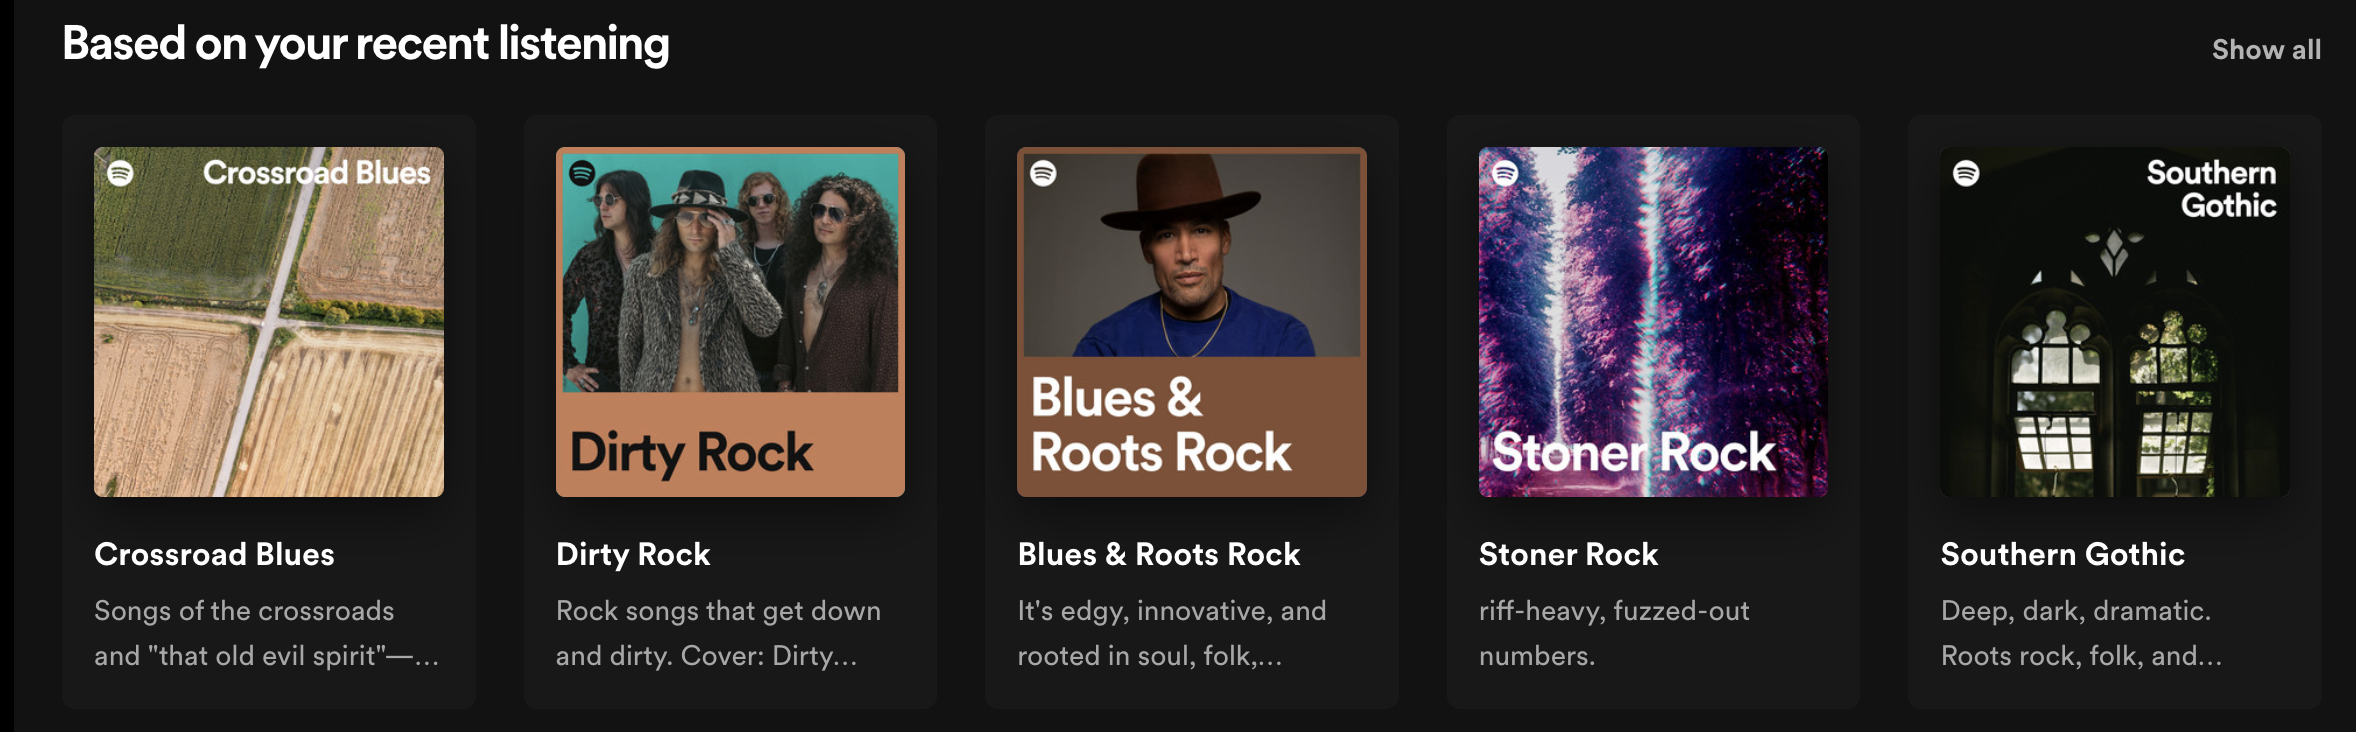
\includegraphics[width=0.8\textwidth]{chapters/chap01/images/spotify.png}
    \caption{Recomendações de \textit{playlists} no Spotify em Agosto de 2023.}
    \label{fig:spotify}
\end{figure}


Personalização é o processo de coleta e uso de informações pessoais para filtrar
conteúdo de forma única a um usuário, atendendo suas necessidades percebidas
pelo serviço ou declaradas explicitamente. \cite{liang2006personalized}.
Recomendações não-personalizadas distribuem o conteúdo recomendado de maneira
igualitária para todos os usuários, desconsiderando suas preferências
individuais. Uma recomendação a partir da lista de reportagens mais lidas em um
portal de notícias é um exemplo de recomendação não-personalizada.
\cite{falk2019practical}.

\begin{figure}[ht]
    \centering
    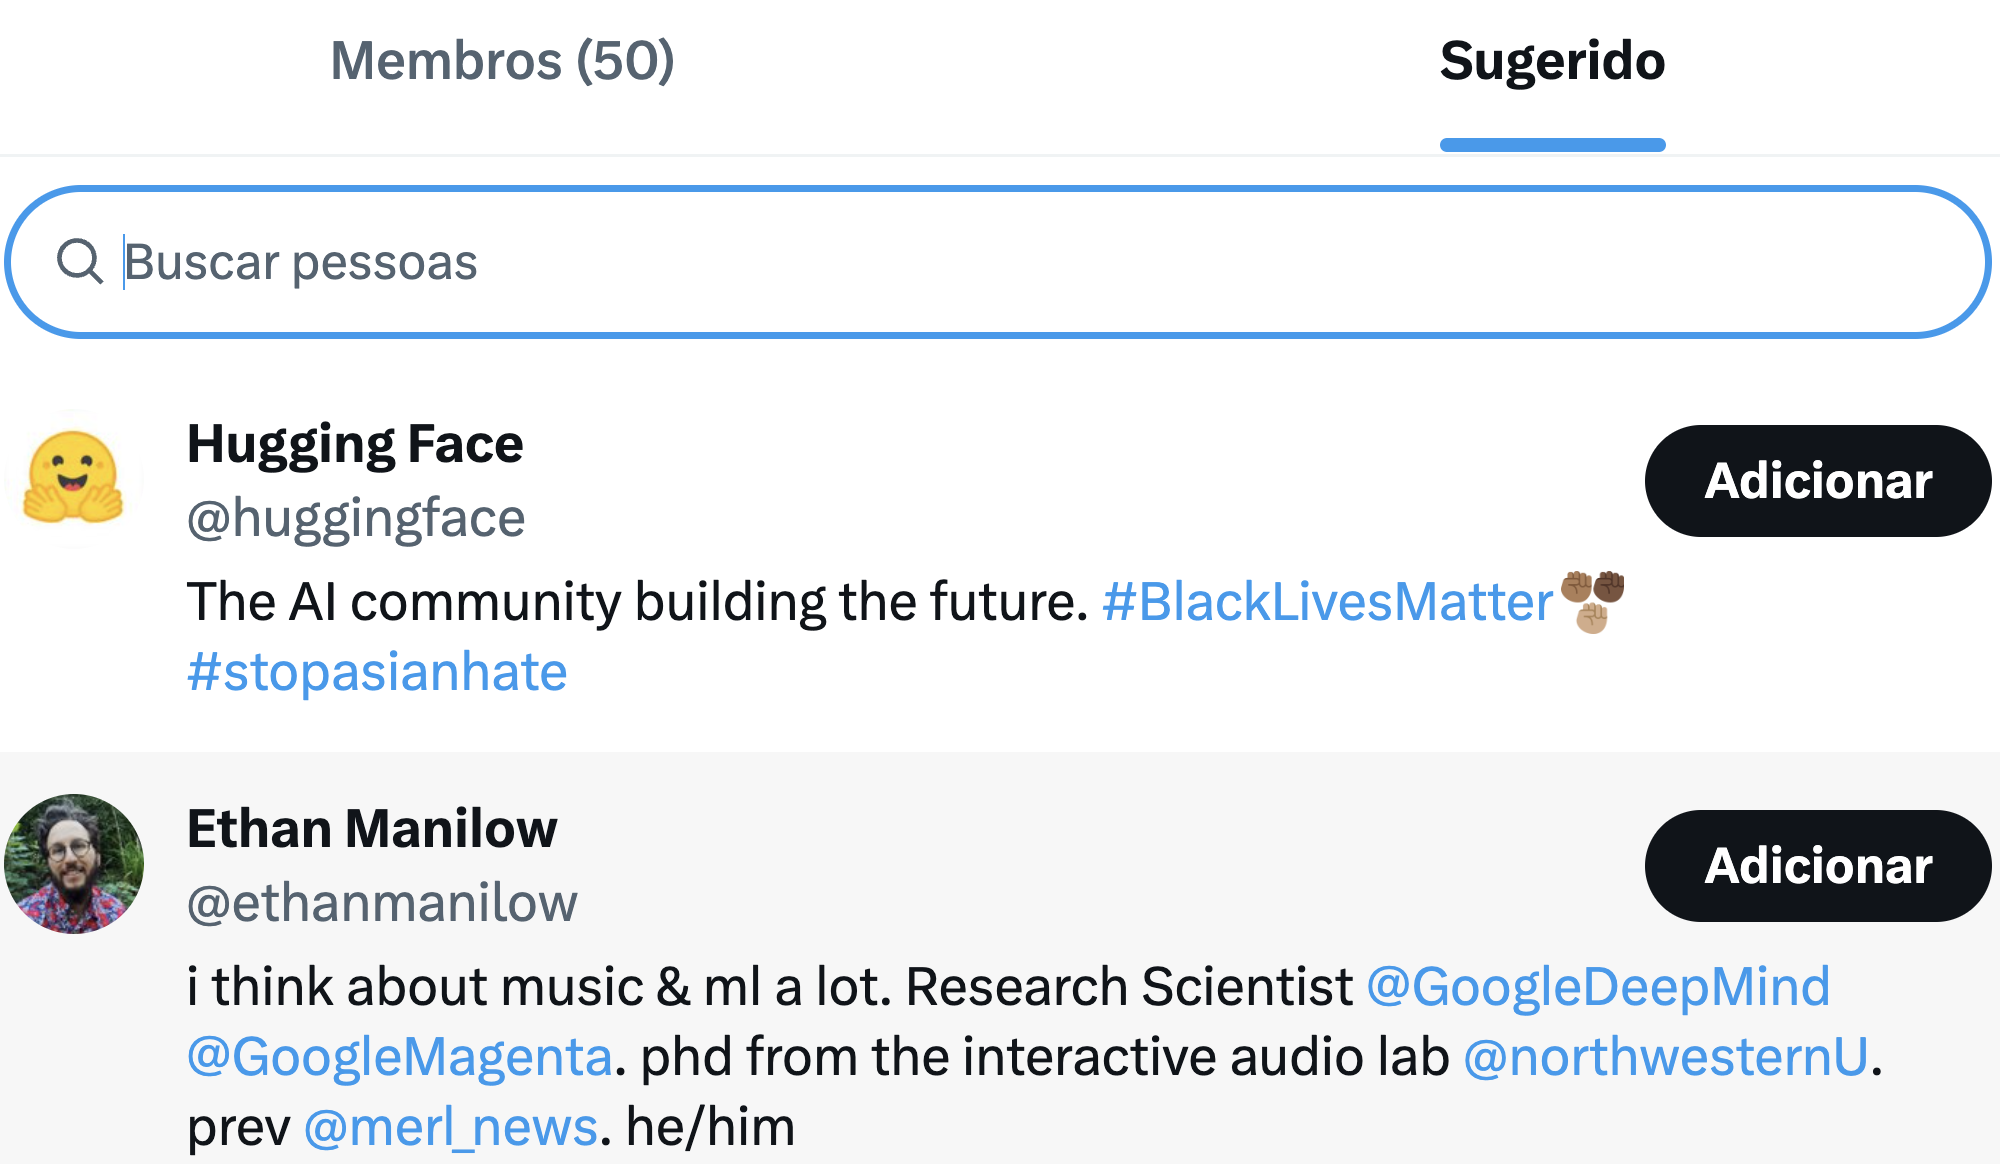
\includegraphics[width=0.6\textwidth]{chapters/chap01/images/tt.png}
    \caption{Recomendações de perfis de usuário no Twitter em Agosto de 2023.}
    \label{fig:twitter}
\end{figure}

% Sistemas de Recomendação Baseados em Sessão (SBRS, do inglês
% \textit{session-based recommender systems}) são sistemas de recomendação que 
Abordagens mais tradicionais em sistemas de recomendação modelam as interações
usuário-item na forma de uma matriz esparsa de avaliações. Cada linha da matriz
representa um usuário e cada coluna representa um item.

A tarefa em questão se
resume ao preenchimento dos valores faltantes da matriz, a depender da
abordagem escolhida. Valores preenchidos com avaliações altas são recomendados
ao usuário, uma vez que ele ainda não os consumiu, tal como ilustrado
na FIGURA \ref{fig:matriz_15}.


\begin{figure}[h]
    \centering
    \begin{tikzpicture}
        % Define the matrix
        \matrix (m) [matrix of nodes,
                    %  nodes in empty cells,
                     column sep=-\pgflinewidth,  % Adjust cell spacing
                     row sep=-\pgflinewidth,     % Adjust cell spacing
                     nodes={draw, text width=2.5em, align=center, minimum height=2.5em, minimum width=2.5em}] {
            5 & 4 & 1 & 1 \\
            4 & 4 & 1 & 1 \\
            1 & 2 &  & 4 \\
            1 & 1 & 4 & 4 \\
        };
      
        % % Labels on the left
        \foreach \row/\label in {1/Gilberto, 2/Maria, 3/Gal, 4/Caetano} {
          \node[left] at (m-\row-1.west) {\label};
        }
      
        % % Labels on the top
        \foreach \col/\label in {1/TV, 2/DVD, 3/sal, 4/pipoca} {
          \node[above,
          ] at (m-1-\col.north) {\label};
        }
      \end{tikzpicture}
      \caption{Matriz de avaliações para produtos de um comércio eletrônico. A predição atua sobre as avaliações não preenchidas.}
      \label{fig:matriz_15}
\end{figure}

\abbrev{SBRS}{Sistemas de recomendação baseados em sessão}
Por mais que a matriz de avaliações seja uma forma intuitiva de representação,
viabilizando uma boa variedade de modelos, trata-se de uma forma que
desconsidera o contexto temporal das interações ou a sequência específica de
itens que determinado usuário interagiu. Sistemas de Recomendação Baseados em
Sessão (SBRS, do inglês \textit{session-based recommender systems}) atuam
justamente nesse cenário.

Os SBRS se caracterizam pelos seus dados representarem um conjunto delimitado de
interações obtidas por \textit{feedback} implícito, ou seja, por preferências
indiretas identificadas a partir de ações ou padrões de navegação. Essas interações
são agrupadas em conjuntos denominados sessões. Uma sessão pode conter uma sequência temporalmente
ordenada de ações executadas por um usuário, ou um conjunto de ações executadas
por um usuário anônimo sem uma ordem específica.

Os objetivos de um SBRS incluem
prever a próxima interação do usuário durante uma sessão em andamento,
recomendar o próximo item ou um conjunto de itens para uma sessão, ou ainda
recomendar uma sessão inteira \cite{domingues_large_2023, survey_wang_2021}.


    



\begin{figure}[h]
    \centering
        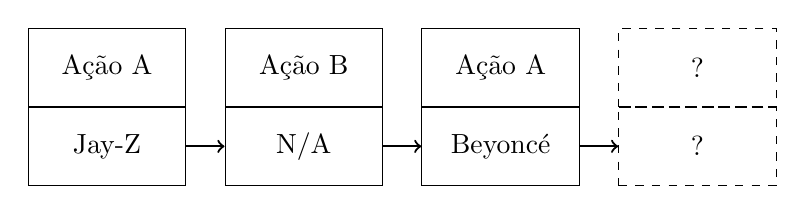
\begin{tikzpicture}
        % Draw the list cells
        \node[draw, rectangle, minimum width=2cm, minimum height=1cm] (cell1) at (0, 0) {Jay-Z};
        \node[draw, rectangle, minimum width=2cm, minimum height=1cm] (cell2) at (2.5, 0) {N/A};
        \node[draw, rectangle, minimum width=2cm, minimum height=1cm] (cell3) at (5, 0) {Beyoncé};
        \node[draw, dashed, rectangle, minimum width=2cm, minimum height=1cm] (cell4) at (7.5, 0) {?};

        % Draw the arrow
        \draw[->, thick] (cell1.east) -- (cell2.west);
        \draw[->, thick] (cell2.east) -- (cell3.west);
        \draw[->, thick] (cell3.east) -- (cell4.west);

        % % Add label to the left of the first cell
        % \node[left] at (cell1.west) {Sessão 1};

        % Draw the top cells with actions
        \node[draw, rectangle, minimum width=2cm, minimum height=1cm] (topcell1) at (0, 1.0) {Ação A};
        \node[draw, rectangle, minimum width=2cm, minimum height=1cm] (topcell2) at (2.5, 1.0) {Ação B};
        \node[draw, rectangle, minimum width=2cm, minimum height=1cm] (topcell3) at (5, 1.0) {Ação A};
        \node[draw, dashed, rectangle, minimum width=2cm, minimum height=1cm] (topcell4) at (7.5, 1.0) {?};

    \end{tikzpicture}
    \caption{Exemplo de uma sessão em andamento, em que a ação A corresponde a navegar ao perfil de determinado artista, enquanto que a ação B corresponde a criar uma \textit{playlist} vazia. Nem toda ação é necessariamente associada a um item. A predição atua sobre a interação subsequente.}
\end{figure}

Cada interação das sessões está associada a tuplas que contém um ou mais dos
seguintes dados: a ação executada, o item alvo da ação, o instante em que a ação
foi executada e o usuário responsável pela ação. Por exemplo, uma sessão pode
representar uma lista ordenada de itens selecionados por um usuário anônimo, ou
uma lista de ações executadas por usuários de uma mesma sessão, sem que essas
ações estejam necessariamente atreladas cada uma a um item. Isso é um aspecto
útil dos SBRS, por prover recomendações em aplicações em que não há
distinção entre usuários, ou quando as preferências de longo prazo de um
usuário novo da plataforma não foram identificadas.
\vspace{0.4cm}